\documentclass{article}
\usepackage{tikz}

\usepackage{esvect}
\usetikzlibrary{positioning,calc}
\begin{document}

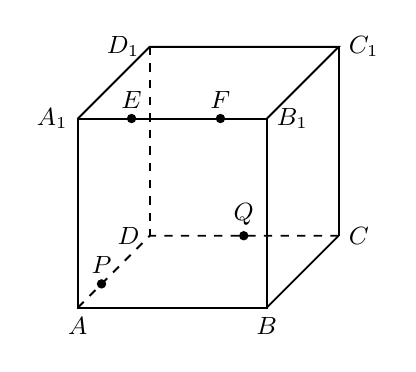
\begin{tikzpicture}[line width=0.7 pt,scale=1.2]
%\draw[help lines] (0,0) grid (3,3);
\draw (0,0) node[below](A) {\small$A$}--(2,0) node[below](B){\small$B$}--(2,2) node[right](B1){\small$B_1$}--(0,2) node[left](A1) {\small$A_1$}--(0,0)--cycle;
\draw[dashed] (0,0)--(0.76,0.76) node[left](D){\small$D$}--(2.76,0.76) node[right](C){\small$C$};
\draw (2.76,0.76)--(2,0);
\draw (0,2) --(0.76,2.76)node[left](D1){\small$D_1$}--(2.76,2.76)node[right](C1){\small$C_1$}--(2,2);
\draw [dashed](0.76,2.76)--(0.76,0.76) ;
\draw (2.76,2.76)--(2.76,0.76);
%\draw [dashed](0.76,2.76)--(2.38,0.38) node[right](E) {\small$E$};
\coordinate [label=\small$E$](E) at($(A1)!0.33!(B1)$) ;
\coordinate [label=\small$F$](F) at($(A1)!0.7!(B1)$) ;
\coordinate [label=\small$P$](P) at($(0,0)!0.33!(0.76,0.76)$) ;
\coordinate [label=\small$Q$](Q) at($(D)!0.5!(C)$) ;
%\draw[fill] (E) circle (1.1pt);
%\draw[fill] (F) circle (1.1pt);
%\draw[fill] (P) circle (1.1pt);
%\draw[fill] (Q) circle (1.1pt);
\foreach \p in{E,F,P,Q}
\draw[fill](\p) circle(1.1pt);
\end{tikzpicture}
\end{document}